\documentclass[10pt,journal]{IEEEtran}


\usepackage{amsfonts}
\usepackage{amsmath}
\usepackage{algorithm}
\usepackage{algorithmic}
\usepackage{amssymb}
\usepackage{graphicx}
\usepackage{cite}
\usepackage{subfigure}
\usepackage{float}
\usepackage{color}
\usepackage{listings}
\usepackage{pythonhighlight}


\begin{document}


\title{Reverse Engineering Algorithmic Mechanism Behind WeChat Red Envelope}

\author{\IEEEauthorblockN{Qifan Zhang,\ 47422183,\ zhangqf@shanghaitech.edu.cn}\\
\IEEEauthorblockA{School of Information Science and Technology\\
  ShanghaiTech University}} 
\maketitle

\begin{abstract}
	  \emph{WeChat Red Envelope}\ is now becoming a fashion around. We always ask, is it fair for every one participating in this \emph{trying-luck}\ game? This article will look into this problem taking the case that 5 people pick 10 \emph{yuan} as an example.
\end{abstract}


\section{Introduction}
	I give out 10 \emph{yuan} for 5 people each time. Priorly my classmates and I conduct 80 trials to get the prior distribution of money every one gets by sequence of picking red envelopes. Then I guess and build up our model based on the 80 prior trials. Finally, I will test my model by 100 posterior trials.
	\\
	All cell phones used in our experiments are conducted on WeChat 6.6.1 on iOS.
	\\
	The main results and contributions of this report are summarized as follows:
\begin{itemize}
  \item \textbf{Modeling.  }
  \item \textbf{Simulation Verification.}
  \item \textbf{Theoretical Analysis}.    
\end{itemize}


\section{Model and Algorithms}
	From 80 prior cases, we notice that the first participant \textbf{will never get more than \(\frac{2}{5}\) of the total money (i.e. 4 \emph{yuan})}. The distribution and potential PMF curve are showing below:	
	Define money gotten by the \(j\)th participant is \(X_j\).
	\\
%%%%%%%%%%%%%%%%%%%%%%%%%%%%%%%%%%%%%%%%%%%%%%
\begin{figure}[!ht]
	\centering
	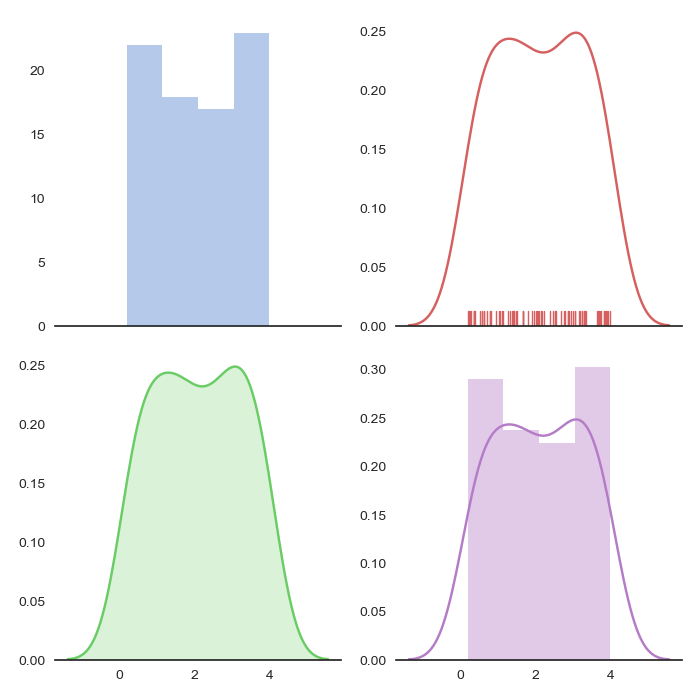
\includegraphics[width=0.7\columnwidth,height=0.6\linewidth]{10_1.png}
	\caption{Distribution of \(X_1\)}
\end{figure}
%%%%%%%%%%%%%%%%%%%%%%%%%%%%%%%%%%%%%%%%%%%%%%
\\
We can see it clearly that no red envelop for the first participant is larger than 4 \emph{yuan}, and from 0 to 4 \emph{yuan}, it distributes nearly uniformly. Ie also found that in a 100-\emph{yuan} red envelop, the first participant could get at most 40 \emph{yuan} and in a 1-\emph{yuan} red envelop, the first participant could get at most 0.4 \emph{yuan}. According to facts above, I model that:
\begin{displaymath}
	X_1\sim Unif(0,\frac{2}{5}\times10)
\end{displaymath}
Then, we guess that every one except the last is following this rule, i.e.
\begin{displaymath}
X_j|X_1,X_2,...,X_{j-1}\sim Unif(0,\frac{2}{5}\times(10-\sum_{i=1}^{j-1}X_i))\ (1\leq j\leq 4)
\end{displaymath}
\(X_5=10-\sum_{i=1}^{4}X_i\)
\\
It does not fit the following prior distributions, but the shape is quite similar:
\\
\begin{figure}[!ht]
	\centering
	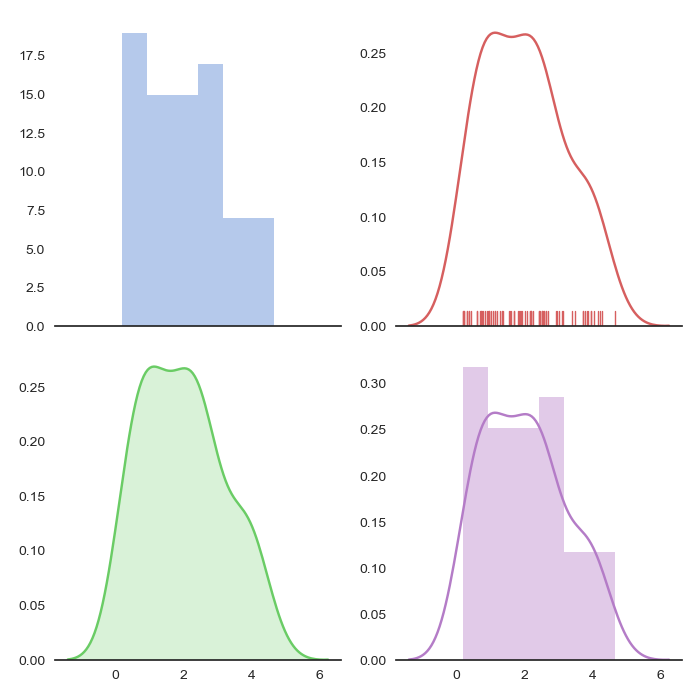
\includegraphics[width=0.7\columnwidth,height=0.6\linewidth]{10_2.png}
	\caption{Distribution of \(X_2\)}
\end{figure}
\begin{figure}[!ht]
	\centering
	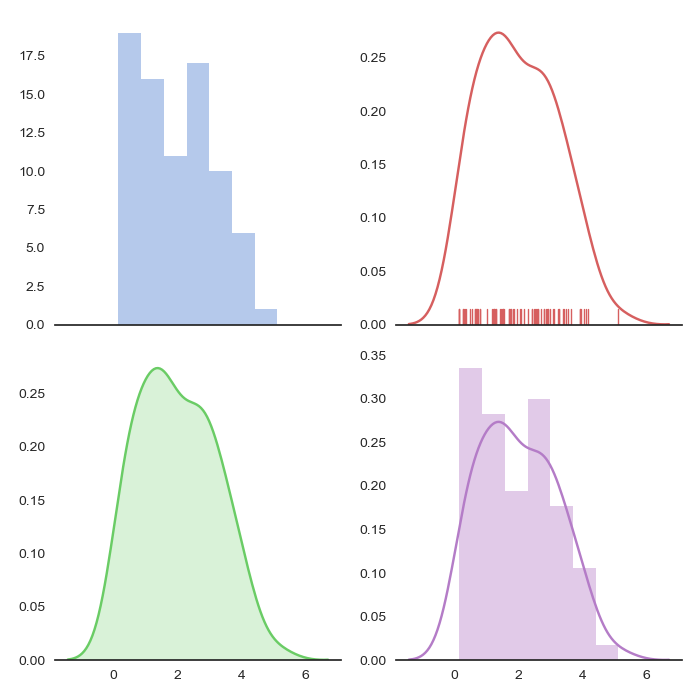
\includegraphics[width=0.7\columnwidth,height=0.6\linewidth]{10_3.png}
	\caption{Distribution of \(X_3\)}
\end{figure}
\begin{figure}[!ht]
\centering
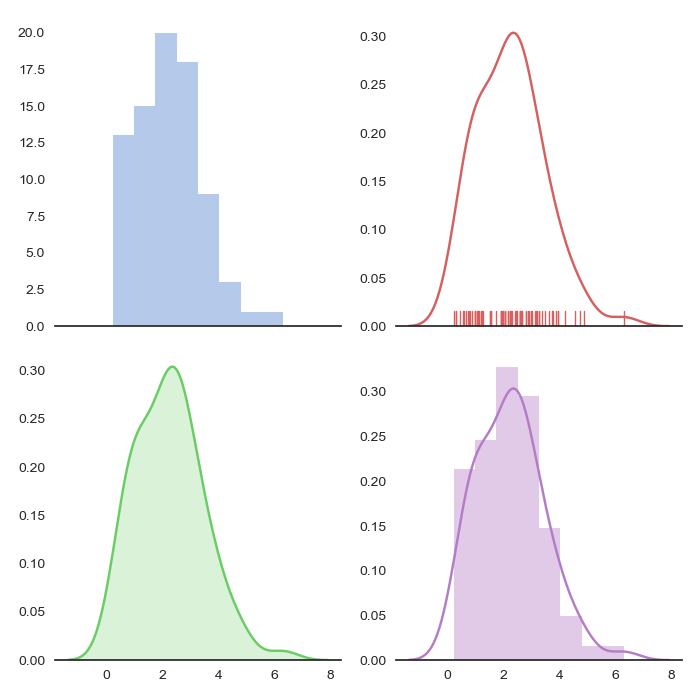
\includegraphics[width=0.7\columnwidth,height=0.6\linewidth]{10_4.png}
\caption{Distribution of \(X_4\)}
\end{figure}
\begin{figure}[!ht]
\centering
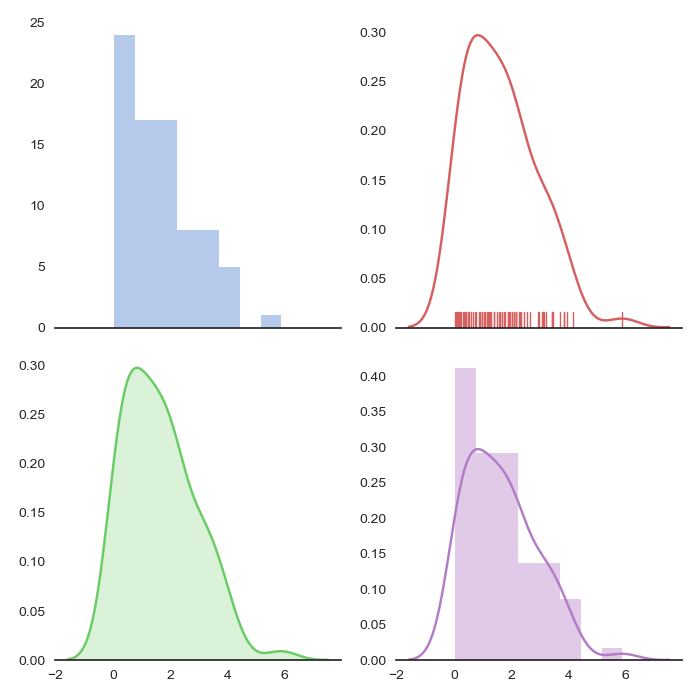
\includegraphics[width=0.7\columnwidth,height=0.6\linewidth]{10_5.png}
\caption{Distribution of \(X_5\)}
\end{figure}
\begin{figure}[!ht]
	\centering
	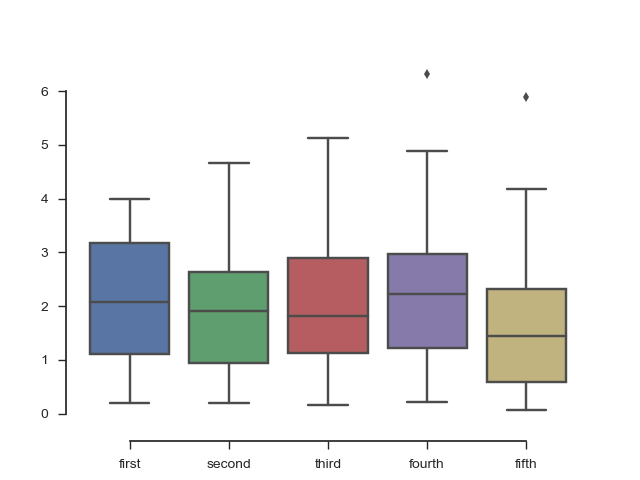
\includegraphics[width=0.7\columnwidth,height=0.6\linewidth]{10_Overall.png}
	\caption{Overall Distribution in one red envelop}
\end{figure}
Therefore, we guess that it follows:
\begin{displaymath}
X_j|X_1,X_2,...,X_{j-1}\sim Unif(0,\frac{2}{6-i}\times(10-\sum_{i=1}^{j-1}X_i))\ (1\leq j\leq 4)
\end{displaymath}
\(X_5=10-\sum_{i=1}^{4}X_i\)
\\
It works well.
\\
Then we generalize the distribution, for a \(n\)-\emph{yuan} red envelop for \(m\)\ participators:
\[
	\begin{split}
		X_1&\sim Unif(0,\frac{2n}{m})
		\\
		X_j|X_1,X_2,...,X_{j-1}&\sim Unif(0,\frac{2(n-\sum_{i=1}^{j-1}X_i)}{m+1-j})
		\\
		&2\leq j\leq m-1
		\\
		X_m&=n-\sum_{i=1}^{m}X_i
	\end{split}
\]

\section{Simulation Results}
I use Python programming language for simulation:
\inputpython{Stimulation_1.py}{1}{20}
I generate 100 cases for a 10-\emph{yuan} red envelop for 5 participators. Results are below:
\\
%%%%%%%%%%%%%%%%%%%%%%%%%%%%%%%%%%%%%%%%%%%%
\begin{figure}[!ht]
	\centering
	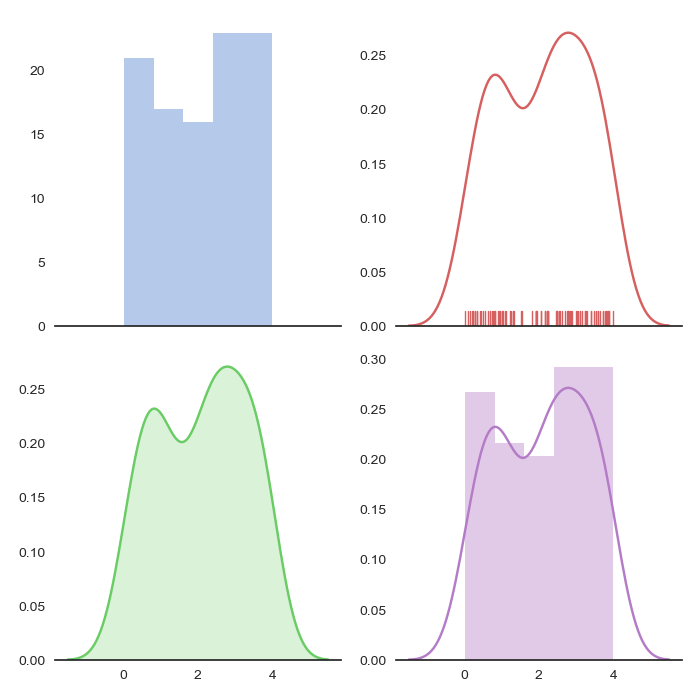
\includegraphics[width=0.7\columnwidth,height=0.6\linewidth]{output_1.png}
	\caption{Distribution of \(X_1\)}
\end{figure}
%%%%%%%%%%%%%%%%%%%%%%%%%%%%%%%%%%%%%%%%%%%%
%%%%%%%%%%%%%%%%%%%%%%%%%%%%%%%%%%%%%%%%%%%%
\begin{figure}[!ht]
	\centering
	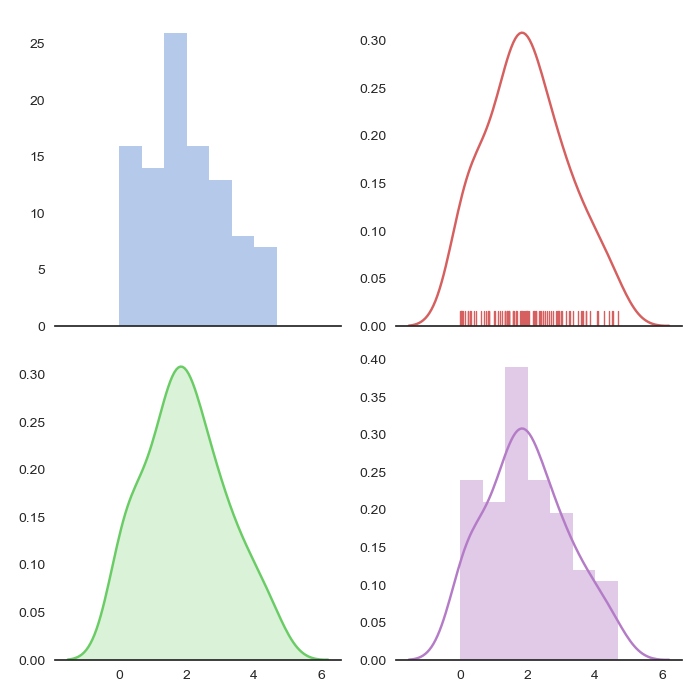
\includegraphics[width=0.7\columnwidth,height=0.6\linewidth]{output_2.png}
	\caption{Distribution of \(X_2\)}
\end{figure}
%%%%%%%%%%%%%%%%%%%%%%%%%%%%%%%%%%%%%%%%%%%%
%%%%%%%%%%%%%%%%%%%%%%%%%%%%%%%%%%%%%%%%%%%%
\begin{figure}[!ht]
	\centering
	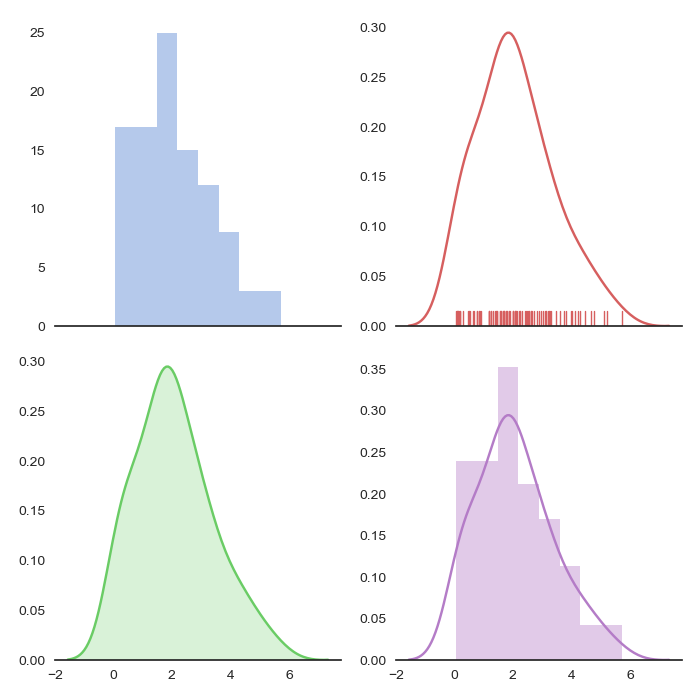
\includegraphics[width=0.7\columnwidth,height=0.6\linewidth]{output_3.png}
	\caption{Distribution of \(X_3\)}
\end{figure}
%%%%%%%%%%%%%%%%%%%%%%%%%%%%%%%%%%%%%%%%%%%%
%%%%%%%%%%%%%%%%%%%%%%%%%%%%%%%%%%%%%%%%%%%%
\begin{figure}[!ht]
	\centering
	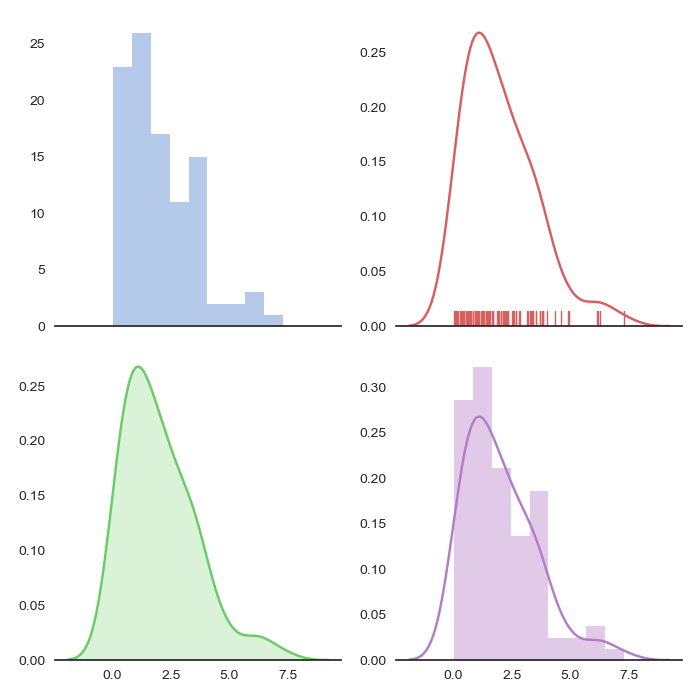
\includegraphics[width=0.7\columnwidth,height=0.6\linewidth]{output_4.png}
	\caption{Distribution of \(X_4\)}
\end{figure}
%%%%%%%%%%%%%%%%%%%%%%%%%%%%%%%%%%%%%%%%%%%%
\pagebreak
%%%%%%%%%%%%%%%%%%%%%%%%%%%%%%%%%%%%%%%%%%%%
\begin{figure}[!ht]
	\centering
	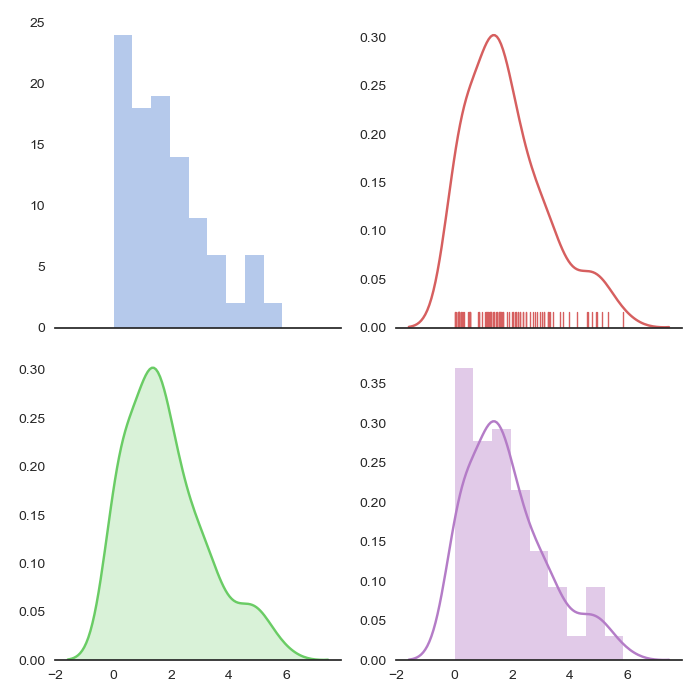
\includegraphics[width=0.7\columnwidth,height=0.6\linewidth]{output_5.png}
	\caption{Distribution of \(X_5\)}
\end{figure}
%%%%%%%%%%%%%%%%%%%%%%%%%%%%%%%%%%%%%%%%%%%%
\begin{figure}[!ht]
	\centering
	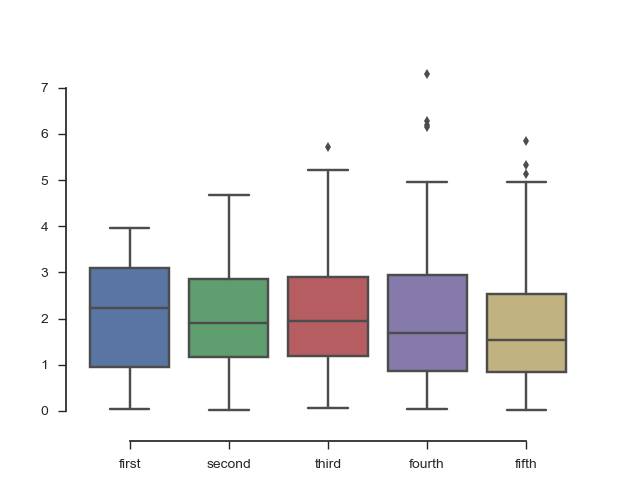
\includegraphics[width=0.7\columnwidth,height=0.6\linewidth]{output.png}
	\caption{Overall Distribution in one red envelop}
\end{figure}
\\
\pagebreak
\section{Result Analysis}
In order to compare with my stimulation results with real ones, I do 20 more real trials combined with previous 80 trials as posterior verification.
\\
The results are below:
\begin{figure}[!ht]
	\centering
	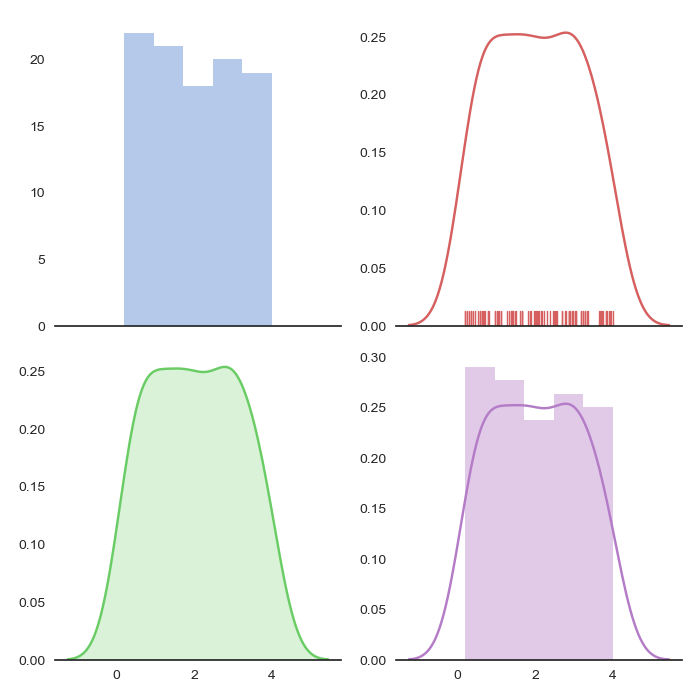
\includegraphics[width=0.7\columnwidth,height=0.6\linewidth]{Posterior_1.png}
	\caption{Distribution of \(X_1\)}
\end{figure}
%%%%%%%%%%%%%%%%%%%%%%%%%%%%%%%%%%%%%%%%%%%%
%%%%%%%%%%%%%%%%%%%%%%%%%%%%%%%%%%%%%%%%%%%%
\begin{figure}[!ht]
	\centering
	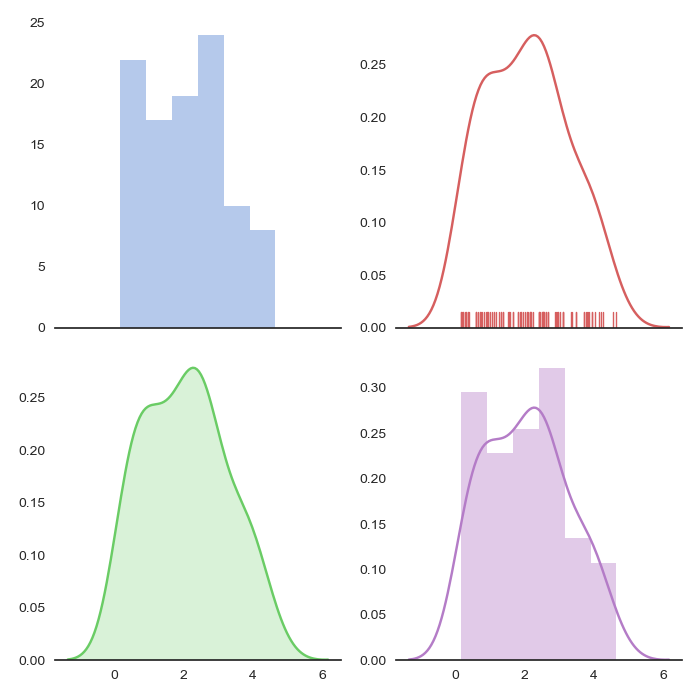
\includegraphics[width=0.7\columnwidth,height=0.625\linewidth]{Posterior_2.png}
	\caption{Distribution of \(X_2\)}
\end{figure}
%%%%%%%%%%%%%%%%%%%%%%%%%%%%%%%%%%%%%%%%%%%%
%%%%%%%%%%%%%%%%%%%%%%%%%%%%%%%%%%%%%%%%%%%%
\begin{figure}[!ht]
	\centering
	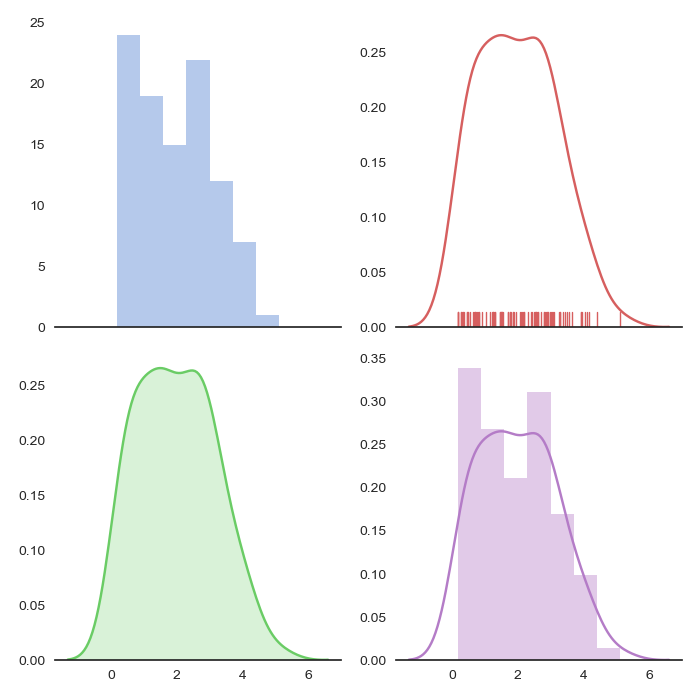
\includegraphics[width=0.7\columnwidth,height=0.525\linewidth]{Posterior_3.png}
	\caption{Distribution of \(X_3\)}
\end{figure}
%%%%%%%%%%%%%%%%%%%%%%%%%%%%%%%%%%%%%%%%%%%%
%%%%%%%%%%%%%%%%%%%%%%%%%%%%%%%%%%%%%%%%%%%%
\begin{figure}[!ht]
	\centering
	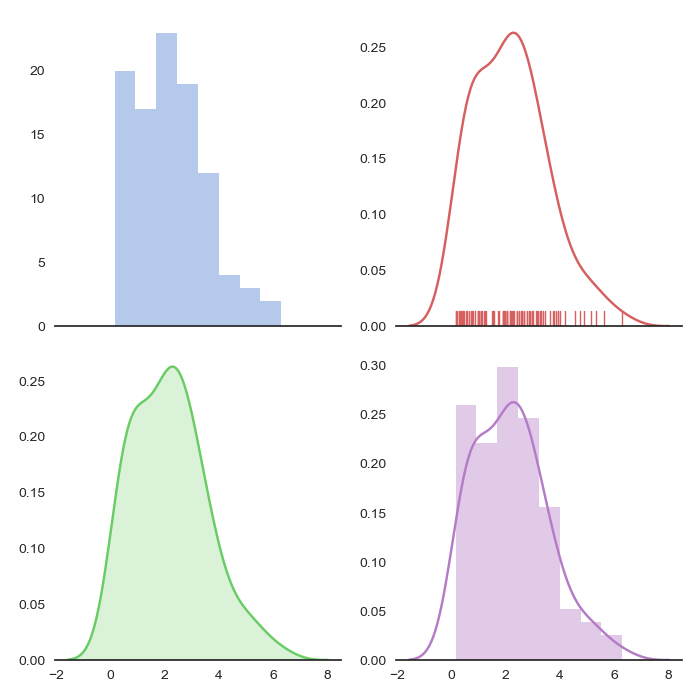
\includegraphics[width=0.7\columnwidth,height=0.525\linewidth]{Posterior_4.png}
	\caption{Distribution of \(X_4\)}
\end{figure}
%%%%%%%%%%%%%%%%%%%%%%%%%%%%%%%%%%%%%%%%%%%%
%%%%%%%%%%%%%%%%%%%%%%%%%%%%%%%%%%%%%%%%%%%%
\begin{figure}[!ht]
	\centering
	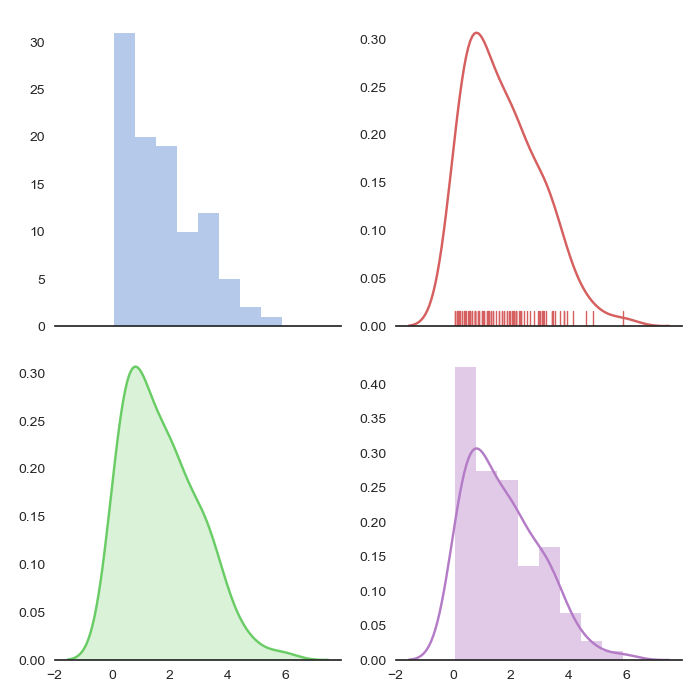
\includegraphics[width=0.7\columnwidth,height=0.5\linewidth]{Posterior_5.png}
	\caption{Distribution of \(X_5\)}
\end{figure}
%%%%%%%%%%%%%%%%%%%%%%%%%%%%%%%%%%%%%%%%%%%%
\begin{figure}[!ht]
	\centering
	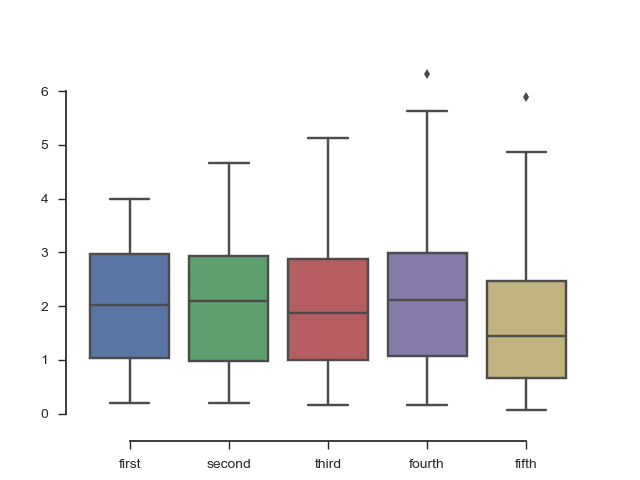
\includegraphics[width=0.7\columnwidth,height=0.6\linewidth]{Posterior.png}
	\caption{Overall Distribution in one red envelop}
\end{figure}
\pagebreak
Intuitively, my model satisfies real trials very well.
\\
Assuming that my model is right, I conduct 1 million times stimulation trials. Since 1 million is large, we see it as the whole of the distribution. \textbf{Fig.19} below shows its overall mean and variance.
\\
\begin{figure}[!ht]
	\centering
	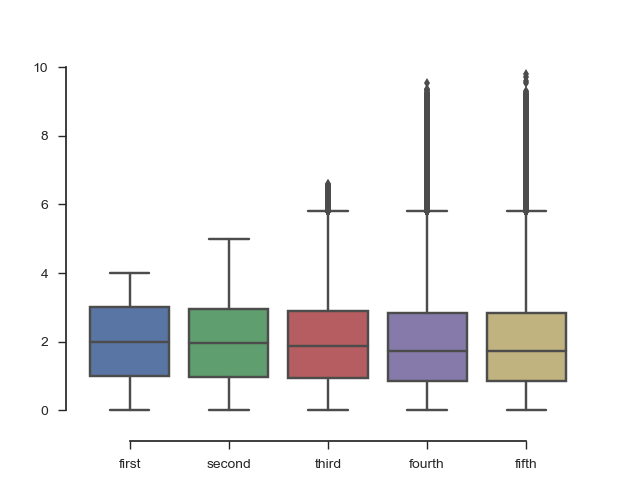
\includegraphics[width=0.7\columnwidth,height=0.8\linewidth]{Stimulation.png}
	\caption{Distribution of \(X_5\)}
\end{figure}
It could be seen that the mean of money every one gets is 2 with variance becoming larger and larger.
\\
From \emph{Standard Deviation of Probability Distribution}:
\[
	\begin{split}
		\sigma_X&=\sqrt{Var(X)}
		\\
		&=\lim\limits_{n\rightarrow\infty}\sqrt{\frac{1}{N}\sum_{i=1}^{n}(X_i-\mu)}
		\\
		S&=\sqrt{\frac{1}{N-1}\sum_{i=1}^{n}(X_i-\mu)}
	\end{split}
\]
Compare the 1 million stimulation model with real trials, we could see that the third, fourth and fifth participants suffer more unstable distributions, which meets our expectation from the theory \emph{Standard Deviation of Probability Distribution}. We can also see that the sharps of the distributions are quite similar with the real ones. In all,it is a good model for red envelope distribution.
\section{Conclusions}
Just like my model, define \(X_j\)\ as the money the \(j\)th participant gets for a \(n\)-\emph{yuan} red envelop for \(m\)\ participators. The distribution is:
\[
	\begin{split}
		X_1&\sim Unif(0,\frac{2n}{m})
		\\
		X_j|X_1,X_2,...,X_{j-1}&\sim Unif(0,\frac{2(n-\sum_{i=1}^{j-1}X_i)}{m+1-j}
		\\
		&2\leq j\leq m-1
		\\
		X_m&=n-\sum_{i=1}^{m}X_i
	\end{split}
\] 
Furthermore, from our model, we can learn that mean \(E(X_j)\) for each participator is the same. But variance \(Var(X_j)\)\ gets larger with serial numbers.

\section*{Acknowledgment}
During this project, I collaborated and discussed with my classmates Cheng'an Wang, Huifan Zhang, and Letong Wang. Data of real trials are collected by Cheng'an Wang, Huifan Zhang and me. I got inspiration of \emph{Uniform Distribution} from Zhihu\(\left[ 1 \right]\) and Zybuluo.com\(\left[ 2 \right]\). I think the idea \emph{Uniform Distribution} is quite excellent, but the author does not choose a right domain for it. All the resources of this report have been pushed to Github\(\left[ 3 \right]\).



%\bibliographystyle{IEEEtran}
%\bibliography{Reference}
\section*{Reference}
\(\left[ 1\right]\)\ https://www.zhihu.com/question/22625187/answer/85530416
\\
\(\left[ 2\right]\)\ "Brief Introduction to Framework Design of WeChat Red Envelope" https://www.zybuluo.com/yulin718/note/93148
\\
\(\left[ 3\right]\)\ https://github.com/KevinZhang199803/SI140\_Final\_Project
\end{document}


